\chapter{Appendix: Statistics Background}\label{chapter:stats}

Much of the material presented in this thesis requires an understanding of a few key areas of statistics. This material is typically covered in almost any introductory level statistics course, but is generally not part of the standard undergraduate physics curriculum. For this reason, I've collected some of the key concepts in this section, to potentially serve as a starting point for people who may not already be familiar with the statistical underpinnings of recent source searches in neutrino astronomy. An interactive ipython notebook showing examples of these concepts can also be found as part of the materials for the 2019-2021 IceCube bootcamps\footnotemark.

\footnotetext{https://events.icecube.wisc.edu/event/105/contributions/1054/}

\section{Estimators}
An estimator is a procedure applied to the data sample which gives a numerical value for a property of the parent population, or, as appropriate, a property or parameter of the parent distribution function.

This is a general definition: The sample of interest may have been drawn from a large parent population, for which some property is to be inferred. Alternatively, it may have been generated from a distribution function, arising from a basic law being investigated. This distribution function also has parameters and properties, which one may also wish to calculate (e.g. $\sigma$ for a 1 dimensional gaussian distribution).

Estimators are generally not classified as "right" or "wrong", rather we tend to classify estimators as "good" or "bad" based on their properties. Some properties that are often relevant when describing estimators:

\begin{itemize}
    \item An estimator is \textit{consistent} if it tends to the true value as the number of data values tends to infinity.
    \item An estimator is \textit{unbiased} if its expectation value is equal to the true value.
    \item An estimator is \textit{efficient} if its variance is small.
\end{itemize}

Estimators can be any number of the above, but good estimators should fulfill all three descriptions \cite{barlow_1989}. 

\section{Likelihoods}
One class of estimators that is commonly used in neutrino astronomy are \textit{likelihood-based estimators}. For a set of data, {$x_1, x_2, x_3 ...x_N$} produced from some underlying distribution with parameter $a$, the probability of obtaining that particular data set is the product of the individual probabilities of obtaining each of the $x_i$. This product is referred to as the *likelihood* (eq. \ref{likelihoodeq1} and \ref{likelihoodeq2}):

\begin{equation}
    L(x_1, x_2, x_3..x_N, a) = P(x_1;a)P(x_2;a)...P(x_N;a)
\label{likelihoodeq1}
\end{equation}

\begin{equation}
    L(x_1, x_2, x_3..x_N, a) = \prod_{i=1}^N P(x_i;a)
\label{likelihoodeq2}
\end{equation}

The likelihood is typically used to fit the model parameter $a$, given some observed data {$x_1, x_2, x_3 ...x_N$} by finding the value of $a$ which maximizes the likelihood function. Note that $a$ can be a vector of values in the case that we have a model with multiple free parameters. For computational reasons, the process of maximizing the likelihood is oftentimes done by minimizing the negative log-likelihood instead. Taking the logarithm of the likelihood function turns the product into a sum, making the derivative more intuitive and easier to work with numerically, and the switch from maximization of the likelihood to minimizing the negative likelihood is purely convention. 

\section{Confidence Intervals}
Suppose we want to know the value of a parameter $X$ and have estimated it from the data, giving result $x$. We know the resolution of our underlying distribution, and thus the variance, $V(x)$ and the standard deviation $\sigma$. Our goal is then to create a "confidence interval": An interval within which there is a $C$ \% chance that a single observation will lie within the interval, where $C$ is our "confidence level". Formally, the confidence interval ($x_-, x_+$) for a given confidence level $C$ obeys the requirement that (eq. \ref{confidenceinterval}):

\begin{equation}
    Prob(x_- \leq x \leq x_+) = \int_{x_-}^{x_+}P(x)dx = C
    \label{confidenceinterval}
\end{equation}

There are a few possible ways to construct this interval:

\begin{enumerate}
    \item The \textbf{symmetric interval}: $x_-$ and $x_+$ are equidistant from the mean, $\mu$, i.e $x_+ - \mu = \mu - x_-$
    \item The \textbf{central interval}: The probability above and below the interval are equal: $\int_{-\infty}^{x_-} P(x)dx = \int_{x^+}^{\infty} P(x)dx = (1-C)/2$
\end{enumerate}

Common values for $C$ are 68\% (1 $\sigma$), 90\% (1.64 $\sigma$), and 99\% (2.58 $\sigma$). There is a trade off between a narrow interval and low confidence. You can say with great confidence that a value will lie within a very wide interval, but if one wants to tie it down more precisely the confidence lessens. 

\section{Hypothesis Testing}
Many problems in science can be reduced to attempting to distinguish between 2 distinct possibilities, where the observed data has different properties under each. In many cases, we are attempting to distinguish between a "null hypothesis", which is used to refer to a "default" model (e.g. the absence of neutrino point sources), and an "alternative hypothesis", which represents the addition of some new physics, model parameter, or disagreement with the "default" case (e.g the presence of neutrino point sources). Statistical hypothesis testing is a framework for comparing these two hypotheses, given some set of observed data.

We can roughly break down the process of hypothesis testing into the following steps:

\begin{enumerate}
    \item State relevant null and alternative hypotheses
    \item State the test statistic
    \item Derive the distribution of the test statistic under the null hypothesis
    \item Select significance level ($\alpha$) at which the null hypothesis will be rejected
    \item Compute an observed test statistic from the data
    \item Calculate a p-value and decide whether to reject the appropriate hypothesis
\end{enumerate}

\subsection{State relevant null and alternative hypotheses}
When constructing an analysis, we should be careful to state the null and alternative hypotheses. Typically, the null hypothesis ($H_o$) refers to a statement or default position that there is no relationship between two phenomena, that there is no signal, or that our current models describe the data well. The alternative ($H_a$) hypothesis usually describes the opposite: that there is a relationship between two phenomena, that there is a signal, or that our models to NOT describe the data well. Here are some example pairs of hypotheses one might encounter when working with IceCube data:

\begin{itemize}
    \item $H_o$: Neutrino event arrival directions are not significantly correlated with the positions of blazars identified in Fermi's 3FGL catalog
    \item $H_a$: Neutrino event arrival directions are correlated with the positions of blazars identified in Fermi's 3FGL catalog
\end{itemize}

\begin{itemize}
    \item $H_o$: A 3-flavor oscillation model describes the IceCube data well
    \item $H_a$: IceCube data is inconsistent with a 3-flavor model
\end{itemize}

It is important to be careful when formulating null and alternative hypotheses so as to not overreach with the claims being made should the alternative hypothesis be accepted. In general, it's best to keep in mind the specifics of how a particular analysis is being constructed, and what the property of the data being measured actually is. For example, in the first pair of hypotheses above, it would be improper for our alternative hypothesis to be "blazars are a source of astrophysical neutrinos" if we were only examining the positions of the 3FGL catalog, which covers only a subset of all observed blazars. 

\subsection{State a test statistic}
A \textit{test statistic} is a quantity derived from the sample, intended to be a numerical summary of a dataset that reduces the data to one value that can be used for hypothesis testing. In general, the test statistic is selected in such a way as to quantify, within observed data, behaviors that would distinguish the null and alternative hypotheses. These are very similar to estimators, and we can oftentimes use estimators as test statistics. 

An important property of the test statistic is that its sampling distribution under the null hypothesis must be calculable either exactly or approximately. There are many types of test statistics that you can use, and what the exact form of the test statistic is will usually be determined by your analysis. One example of a test statistic is the chi-squared test statistic intended to compare counts in an oscillation analysis (eq. \ref{chi2eq}):

\begin{equation}
    \chi^2 = \sum_{i \in {bins}} \frac{(n_i^{\nu+\mu_{atm}} - n_i^{data})^2} {(\sigma_i^{data})^2+(\sigma_{\nu+\mu_{atm,i}})^2} 
    \label{chi2eq}
\end{equation}

Where $\chi^2$ is the test statistic, $i$ refers to bins in zenith and azimuth, $n_i^{\nu+\mu_{atm}}$ and $n_i^{data}$ are the number of events in a particular bin in both simulation and data, and $\sigma_{\nu+\mu_{atm,i}}$  and $\sigma_i^{data}$ are similar the per-bin standard deviations in both simulation and data. This test statistic is used to measure the agreement of the data with a "nominal" model that can be simulated to obtain the values $n_i^{\nu+\mu_{atm}}$ and $\sigma_{\nu+\mu_{atm,i}}$. 

Another example of a commonly used test statistic in neutrino astronomy is the point source likelihood (eq. \ref{psllhr}):

\begin{equation}
    TS = -2 \log(\frac{\mathcal{L}(n_s=0)}{\mathcal{L}(\hat{n}_s)})
    \label{psllhr}
\end{equation}

This is a likelihood ratio test statistic, where $\mathcal{L}$ is a likelihood function that describes how clustered events are near a particular location. In its simplest form, this likelihood has 1 parameter, $n_s$, that describes the number of excess events seen near the location being examined. 

The likelihood ratio is a very powerful test statistic. Given two hypotheses $H_o$ and $H_a(a)$ where $H_o = H_a(\tilde{a})$ (they are \textit{nested} models), then the Neyman-Pearson lemma states that the likelihood ratio test has the strongest statistical power (i.e. correctly reject $H_o$ when $H_1$ is true). This is the case for many point source searches, where the null hypothesis ("There are zero signal events, $n_s$ = 0) is nested in the alternative hypothesis ("There are a nonzero number of signal events, $n_s$ > 0"). 

Note that test statistics are essentially estimators of the alternative hypothesis: a "more extreme" test statistic should correspond to the data being better described by the alternative hypothesis. In fact, most test statistics are in fact based on estimators of some statistical property of the data. The point source test statistic, for example, is based around a likelihood estimator of the number of clustered neutrino events. 

\subsection{Select a significance level at which the null hypothesis will be rejected}
Since in testing our hypothesis, we have two options for our result (accept/reject the null hypothesis), and there are two options for the "actual" state of our null hypothesis (either it is true or it isn't), there are four possible outcomes describing whether we were correct or not:

\begin{center}
 \begin{tabular}{|c || c | c|} 
 \hline
  & $H_o$ rejected     & Accept (Fail to reject) $H_o$ \\ [0.5ex] 
 \hline\hline
 $H_o$ False & Correct & Type II error (false negative) \\ 
 \hline
 $H_o$ True & Type II error (false positive) & Correct \\ [1ex] 
 \hline
\end{tabular}
\end{center}

If you reject a true null hypothesis, then this is a type II error. If you accept a false null hypothesis, then this is a type I error. "Type I" and "type II" are needlessly confusing names, so let's instead refer to these with the more intuitive names "false positive" and "false negative". 

Both types of errors are bound to happen sometimes, but we're typically more concerned with false positives: We don't want to make any claims of discovery when in fact it was simply a background fluctuation. We can control the rate at which this happens with the "significance" of the test ($\alpha$). The \textit{significance} refers to the probability of obtaining a false positive. 

Given a hypothesis test with some test statistic (where we can calculate the distribution of this test statistic under the null hypothesis, see above!), we can divide the range of our test statistic into the acceptance region, containing test statistics less extreme than some pre-defined significance threshold, and the rejection region, containing test statistics more extreme than this threshold. If our observed test statistic falls in the acceptance region, we will accept the null hypothesis to be true. If our observed test statistic falls into the rejection region, we will reject the null hypothesis. 

The probability of a false positive is then simply the integral of our null hypothesis test statistic distribution over the rejection region. This is the "significance" of the test. In principle, we can set the significance of our test to be whatever we want, simply by changing the acceptance and rejection regions. In practice, we typically want to set a high bar for announcing a result (this corresponds to a low significance). In particle physics, the threshold for rejecting the null hypothesis is typically set such that the significance is $2.87 \times 10 ^{-7}$ (the one-sided five sigma threshold). In other disciplines, the convention is different, with social scientists and biologists typically rejecting the null hypothesis at the $.01$ or $.05$ significance level. 

You might sometimes hear significance referred to in units of "sigma" (e.g. "$5 \sigma$" or "$3 \sigma$"). This can be obtained by the process shown in figure \ref{fig:sigmamap}, by mapping the significance to a normal distribution. This simply provides a standardized way of describing how "extreme" the observed significance is: more "sigmas" corresponds to a result that is less likely to be seen under the null hypothesis. 

\begin{figure}[h]
\centering
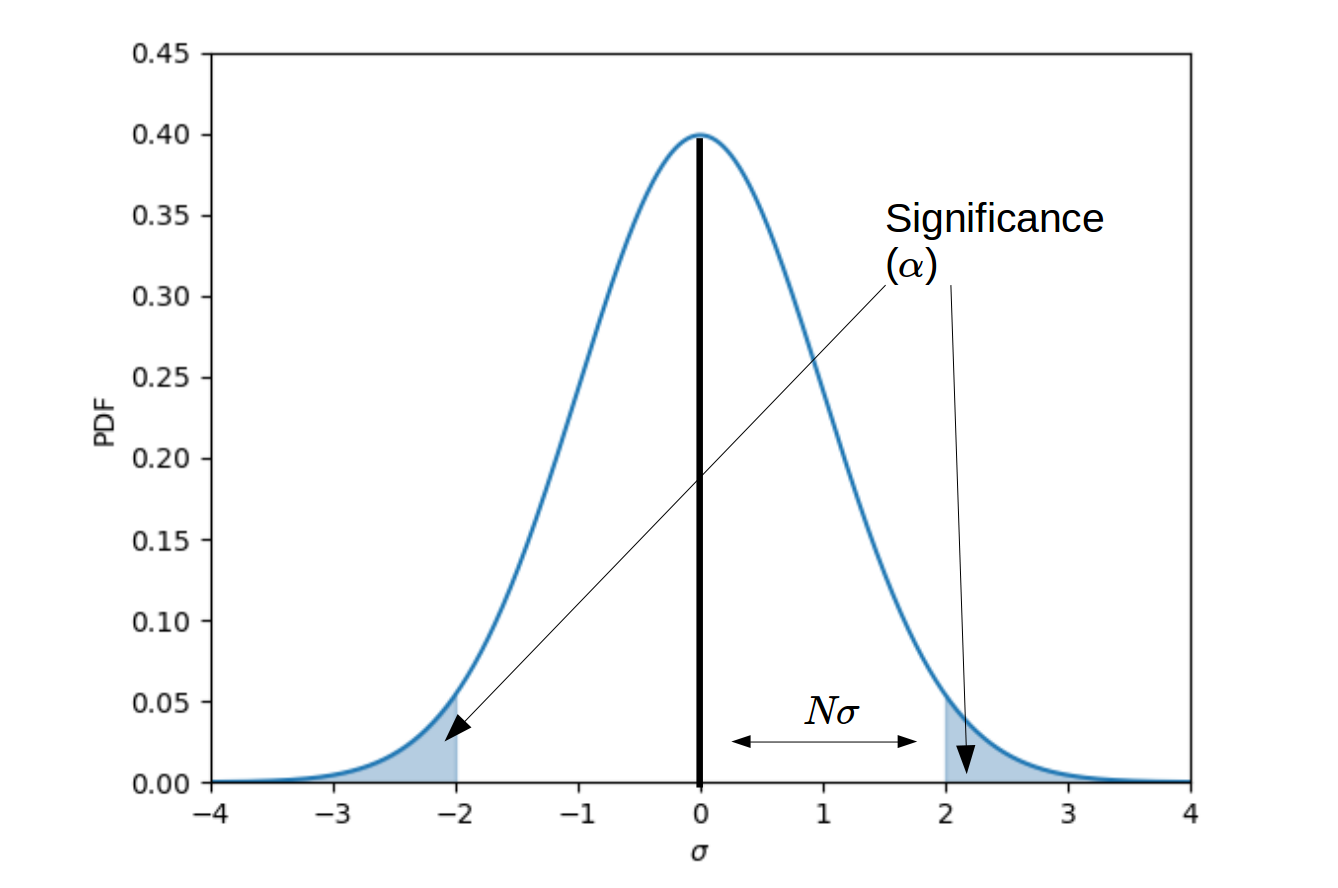
\includegraphics[width=0.8\textwidth]{figs/sigmamap.png}
\caption{The mapping of significance into units of sigma using a normal distribution, for a two tailed test.}
\label{fig:sigmamap}
\end{figure}

\subsection{Compute the TS from observed data}
This step is fairly straightforward, as the test statistic has already been defined. Simply run your test statistic algorithm using the observed data generated from your experimental apparatus. 

\subsection{Decide whether to accept or reject the null hypothesis}
There are two different, but equivalent constructions for deciding whether to reject the null hypothesis or not. The first construction involves pre-defining an \textit{acceptance region} prior to calculating the test statistic associated with the observed data. The acceptance region corresponds to the range of test statistic values for which the null hypothesis cannot be rejected. This is typically chosen to correspond to a particular significance (e.g. 5\%, 1\%, 0.01\% etc.). If the observed test statistic lies outside of the acceptance region corresponding to $X$\% significance, then we can say that the null hypothesis is rejected at the $X$\% significance level. Note that since we had to pick our significance threshold (and consequently define an acceptance region) prior to computing an observed test statistic, we can make no further claims on how extreme the result is: if our acceptance region is $TS > 12$, it does not matter if we observe a $TS = 12.1$ or if we observe a $TS = 99.0$. In both instances we will reject the null hypothesis as the significance level we initially chose. 

An alternative, but mathematically equivalent, construction involves the calculation of a \textit{p-value}. A p-value is the probability, under the null hypothesis, of obtaining a test statistic at least as extreme as the one we have observed from data. If our p-value is smaller than a pre-determined significance threshold, then we can reject the null hypothesis.  The p-value can be calculated by simply integrating our null hypothesis test statistic distribution over the range of values more extreme than what was observed. For the one-tailed case where a larger test statistic is correlated with stronger evidence of the alternative hypothesis, this is (eq. \ref{peq}): 

\begin{equation}
    p = \int_{TS_{obs}}^{\infty} PDF_{H_o}
\label{peq}    
\end{equation}

Where $TS_{obs}$ is our observed test statistic and $PDF_{H_o}$ is the distribution of test statistics under the null hypothesis. It is important to note that the above equation is only valid for the positive, one-tailed case (the alternative hypothesis is only associated with test statistic values on one side of the distribution). A more general formula could be expressed as (eq. \ref{peq_general}):

\begin{equation}
    p = \int_{R|TS_{obs}} PDF_{H_o}
\label{peq_general}    
\end{equation}

Where here $R|TS_{obs}$ is the rejection region of the test statistic distribution associated with a particular observed test statistic (i.e. it is the region of the background test statistic distribution containing values more extreme than what was observed). This distinction is particularly important when conducting two-tailed tests, where test statistics that are either above an upper bound, or below a lower bound may be cause for rejecting the null hypothesis. 

\section{Trial Factors}
Each time you obtain the answer of an analysis from real data, you have done one experimental trial. It is common to perform multiple trials when working with a specific analysis technique.

\begin{itemize}
    \item In the neutrino sources group, we might test the probability that one location is consistent with background expectation. If we were to apply this framework to a list of 30 source candidate locations, then this would be 30 trials.
    \item Repeating an analysis with new cuts. We might count the number of neutrinos with E $>$ 1 TeV in 1 year, then count the number of neutrinos with E $>$ 10 TeV in 1 year. This would be 2 trials. 
    \item Repeating with different signal hypotheses. You might look for emission from blazars using both the hypothesis of steady emission and a flare hypothesis (2 trials)
\end{itemize}
Trials can be both independent, or correlated:

\begin{itemize}
    \item \textbf{Independent}: Search for a new source/signal in 1 year of data, repeat the search in the next year of data (separately). This would be 2 independent trials, as the results of the first year will not affect the results of the second year
    \item \textbf{Correlated}: Search for a new source/signal in 1 year of data, repeat the search with 2 years of data, including the first year. This would be 2 trials, but they would be correlated, since the results of the first 2 years of data will be affected by the results of the first year alone. 
\end{itemize}

Accounting for trials is important, as given enough trials even the null hypothesis can produce a significant result. A simple and conservative way to account for trials is to assume that trials are uncorrelated and apply the Sidak correction (eq. \ref{sidak}):

\begin{equation}
    P_{post} = 1-(1-P_{pre})^N
\label{sidak}
\end{equation}

Where $P_{post}$ is the trial-corrected p-value, $P_{pre}$ is the smallest p-value observed across all trials performed, and $N$ is the number of trials. This formula is intended to describe uncorrelated trials, however it can also be used to obtain a conservative trial correction for correlated trials as well. More sophisticated methods of accounting for correlated trials typically involve simulation of the null hypothesis, and are oftentimes specific to a particular experiment. 

When reporting a trial corrected p-value, it is additionally important to specifically state which trials are being accounted for. Accounting for trials across all sources in a catalog will result in a different p-value than accounting for all analyses performed by the IceCube collaboration, yet both are "post-trial" p-values. 

